
%%
%% -----------------------------------
%%
%% This is a generated file.
%%
%% Copyright (C)
%%       2010 -- 2015 by Zhaoli Wang
%%       2014 -- 2019 by Liam Huang
%%       2019 -- present by latexstudio.net
%%
%% This work may be distributed and/or modified under the
%% conditions of the LaTeX Project Public License, either version 1.3
%% of this license or (at your option) any later version.
%% The latest version of this license is in
%%   http://www.latex-project.org/lppl.txt
%% and version 1.3 or later is part of all distributions of LaTeX
%% version 2005/12/01 or later.
%%
%% This work has the LPPL maintenance status `maintained'.
%%
%% The Current Maintainer of this work is Liam Huang.
%%
%%
%% This is file `mcmthesis-demo.tex',
%% generated with the docstrip utility.
%%
%% The original source files were:
%%
%% mcmthesis.dtx  (with options: `demo')
%%
%% -----------------------------------
%%
%% This is a generated file.
%%
%% Copyright (C)
%%       2010 -- 2015 by Zhaoli Wang
%%       2014 -- 2019 by Liam Huang
%%       2019 -- present by latexstudio.net
%%
%% This work may be distributed and/or modified under the
%% conditions of the LaTeX Project Public License, either version 1.3
%% of this license or (at your option) any later version.
%% The latest version of this license is in
%%   http://www.latex-project.org/lppl.txt
%% and version 1.3 or later is part of all distributions of LaTeX
%% version 2005/12/01 or later.
%%
%% This work has the LPPL maintenance status `maintained'.
%%
%% The Current Maintainer of this work is Liam Huang.
%%

\documentclass{hci}
\usepackage{listings} 
\usepackage{xcolor}
\usepackage{color}
\usepackage{xcolor}
\usepackage{indentfirst}
%%\usepackage{CTeX}
\setlength{\parindent}{2em}
\pmsetup{CTeX = false,   % 使用 CTeX 套装时,设置为 true
        tcn = 1854116 Mingzhi Zhu, 
        sheet = true, titleinsheet = true, keywordsinsheet = true,
        titlepage = true, abstract = true}
\usepackage{newtxtext}%\usepackage{palatino}
\usepackage{lipsum}
%\usepackage[notref,notcite]{showkeys}
\title{Lab 3:Data Visualization}
\author{1854116 
	\\Mingzhi Zhu}
\date{Base on Google Play Store Dataset\\\today}
\definecolor{dkgreen}{rgb}{0,0.6,0}
\definecolor{gray}{rgb}{0.5,0.5,0.5}
\definecolor{mauve}{rgb}{0.58,0,0.82}

\begin{document}

\maketitle
\tableofcontents
\newpage
%% Generate the Table of Contents, if it's needed.
%% \tableofcontents
%% \newpage
%%
%% Generate the Memorandum, if it's needed.
%% \memoto{\LaTeX{}studio}
%% \memofrom{Liam Huang}
%% \memosubject{Happy \TeX{}ing!}
%% \memodate{\today}
%% \logo{\LARGE I'm pretending to be a LOGO!}
%% \begin{memo}[Memorandum]
%%   \lipsum[1-3]
%% \end{memo}
%%
\section{Data Analysis Task}
In this section,report mainly describes a data analysis task for the chosen dataset Google-Play-Store-Dataset. 
\subsection{Dataset Overview}
Google App Store has hundreds of thousands of software on the shelves, and the number of downloads has exceeded 2 billion times. For the majority of Android mobile phone users, it provides a very wide range of application options, which is very popular with users. More than 20000 pieces of music, free and paid,more than 450000 Android applications and games,the largest e-book market in the world.You can rent thousands of movies, including the latest movies and HD movies.Therefore, the app data in Google play story is more typical and comprehensive. Through the analysis of APP related data, it is helpful for domestic companies in the production and operation of app.The structure of the data in the table is as follows in figure1.
\begin{figure}[htbp]
	\centering
	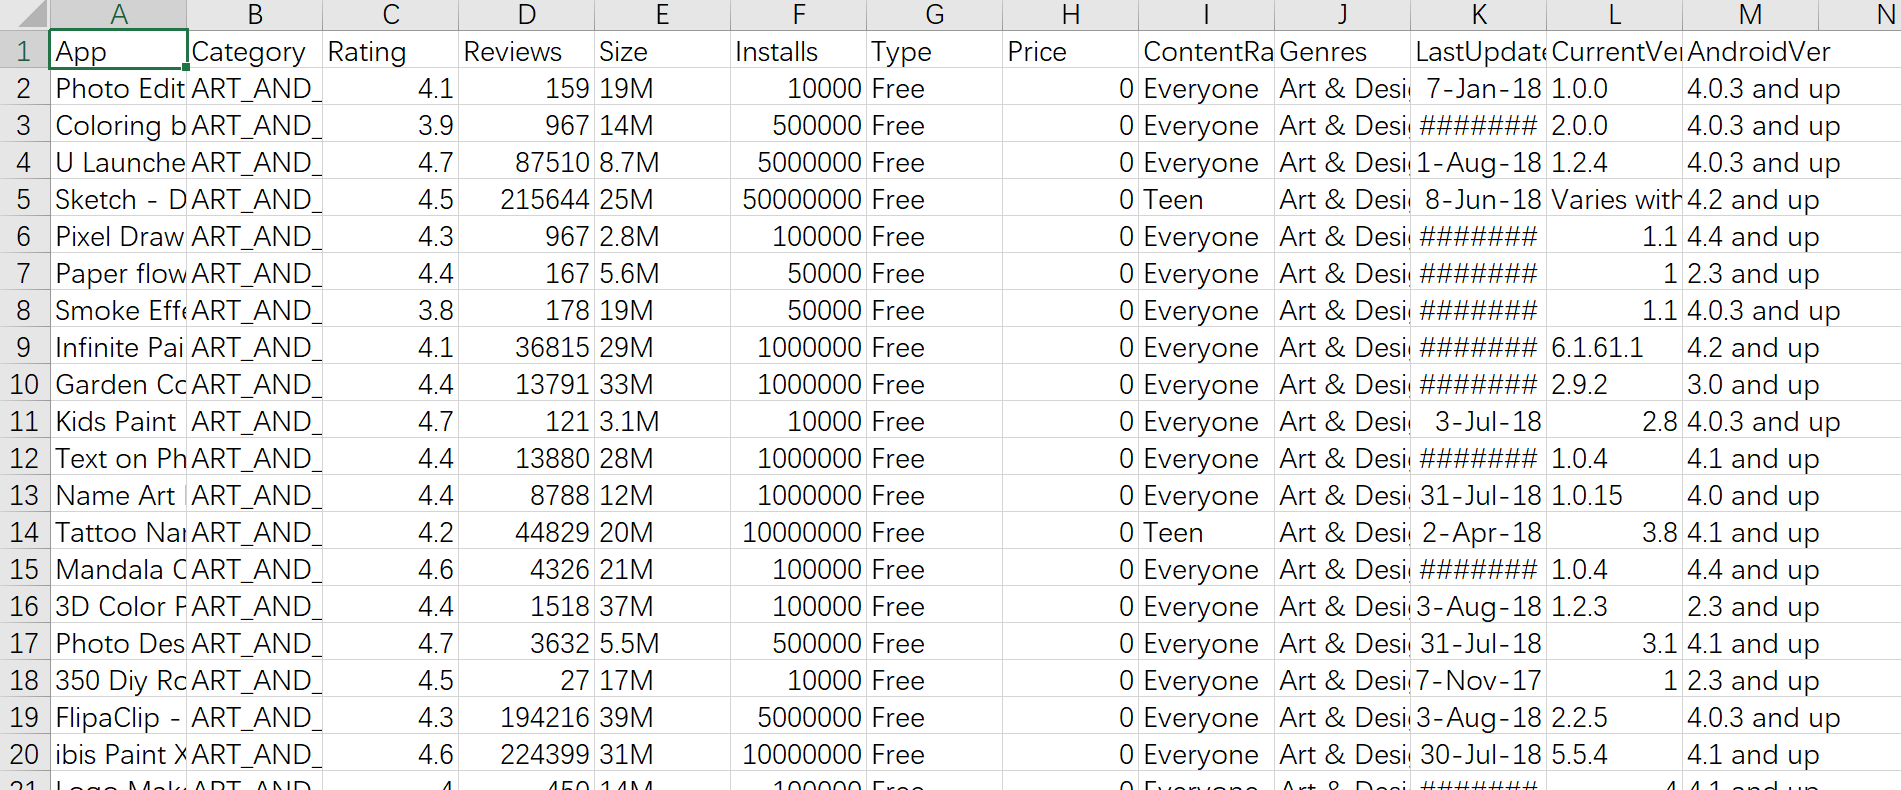
\includegraphics[width=0.8\linewidth]{figures/overview}
	\caption{Data Structure}
	\label{fig:overview}
\end{figure}

The first step in data analysis is to have an overview of the dataset.This dataset records all the apps in Google App Store at that time and has 10840 rows with 13 columns.Thirteen attribute columns record the name, category,rating,application size,downloads and other information of these apps.Aftering overviewing all the dataset,I find there are some  missing values in the dataframe.The relationship between missing values and columns is shown in the table1 below. For the convenience of the final presentation, I have deleted all the rows that contain missing values.After the data preprocessing, the dataset still has 9359 rows.
\begin{table}[htbp] %开始一个表格environment,表格的位置是h,here。  
	\caption{Relationship between Columns and Missing Values} %显示表格的标题
	\centering
	\label{t1}
	\begin{tabular}{c|c} %设置了每一列的宽度,强制转换。 
		\hline
		\hline
		Column Name& Missing Data Number                                                                                                                                         \\

		\hline App&0\\
		\hline	Category &0\\
		\hline	Rating   &1474\\
		\hline	Reviews &0\\
		\hline	Size &0\\
		\hline	Installs &0\\
		\hline	Type &1\\
		\hline	Price &0\\
		\hline	ContentRating &0\\
		\hline	Genres &1\\
		\hline	LastUpdated&0\\
		\hline	CurrentVer &8\\
		\hline	AndroidVer &2\\		
		\hline
	\end{tabular}
\end{table}

\subsection{Objectives}
I choose Google-Play-Store dataset as the data source of my data visualization experiment.
In this dataset I want to know the relation between the \textbf{Rating} and \textbf{Reviews}, the\textbf{ Size of the App} and \textbf{Installs}, the \textbf{Price of the App} and \textbf{Total Number of the Apps} which the price in below this price.

I also want to know the relationship between the data in different app category.For example, I want to know the
characteristics of the Apps which are belong to BUSINESS category.By dividing apps into several subclasses by category attributes,I can hold a global view of the information in the Google Play Store.

Therefor,I picked out the following columns from the original dataset:App,Category,
Rating,Reviews,Size,Installs,Price,Content Rating.

\subsection{Characteristics}
The first thing I have to do is that I should know the characteristic of each attributes and the basic relationship
between different attributes before plotting my data on dashboard.
The dataprocess.py is the script which I write to fetch the attributes I need and use to process data aim to fit the frontend and can show in the dashboard. 
The characteristics of all the attributes I used are list here:
\subsubsection{Category}
\begin{figure}[htbp]
	\centering
	\includegraphics[width=0.8\linewidth]{figures/CountApps}
	\caption{Count of App in Each Category}
	\label{fig:Count}
\end{figure}
Category has 33 different values,and it can be seen that family and game have the largest number of apps.

\subsubsection{Relationship}
The following figure shows each attribute (Rating;Size;Installs;Reviews;Price) scatter plot of each other:
\begin{figure}[htbp]
	\centering
	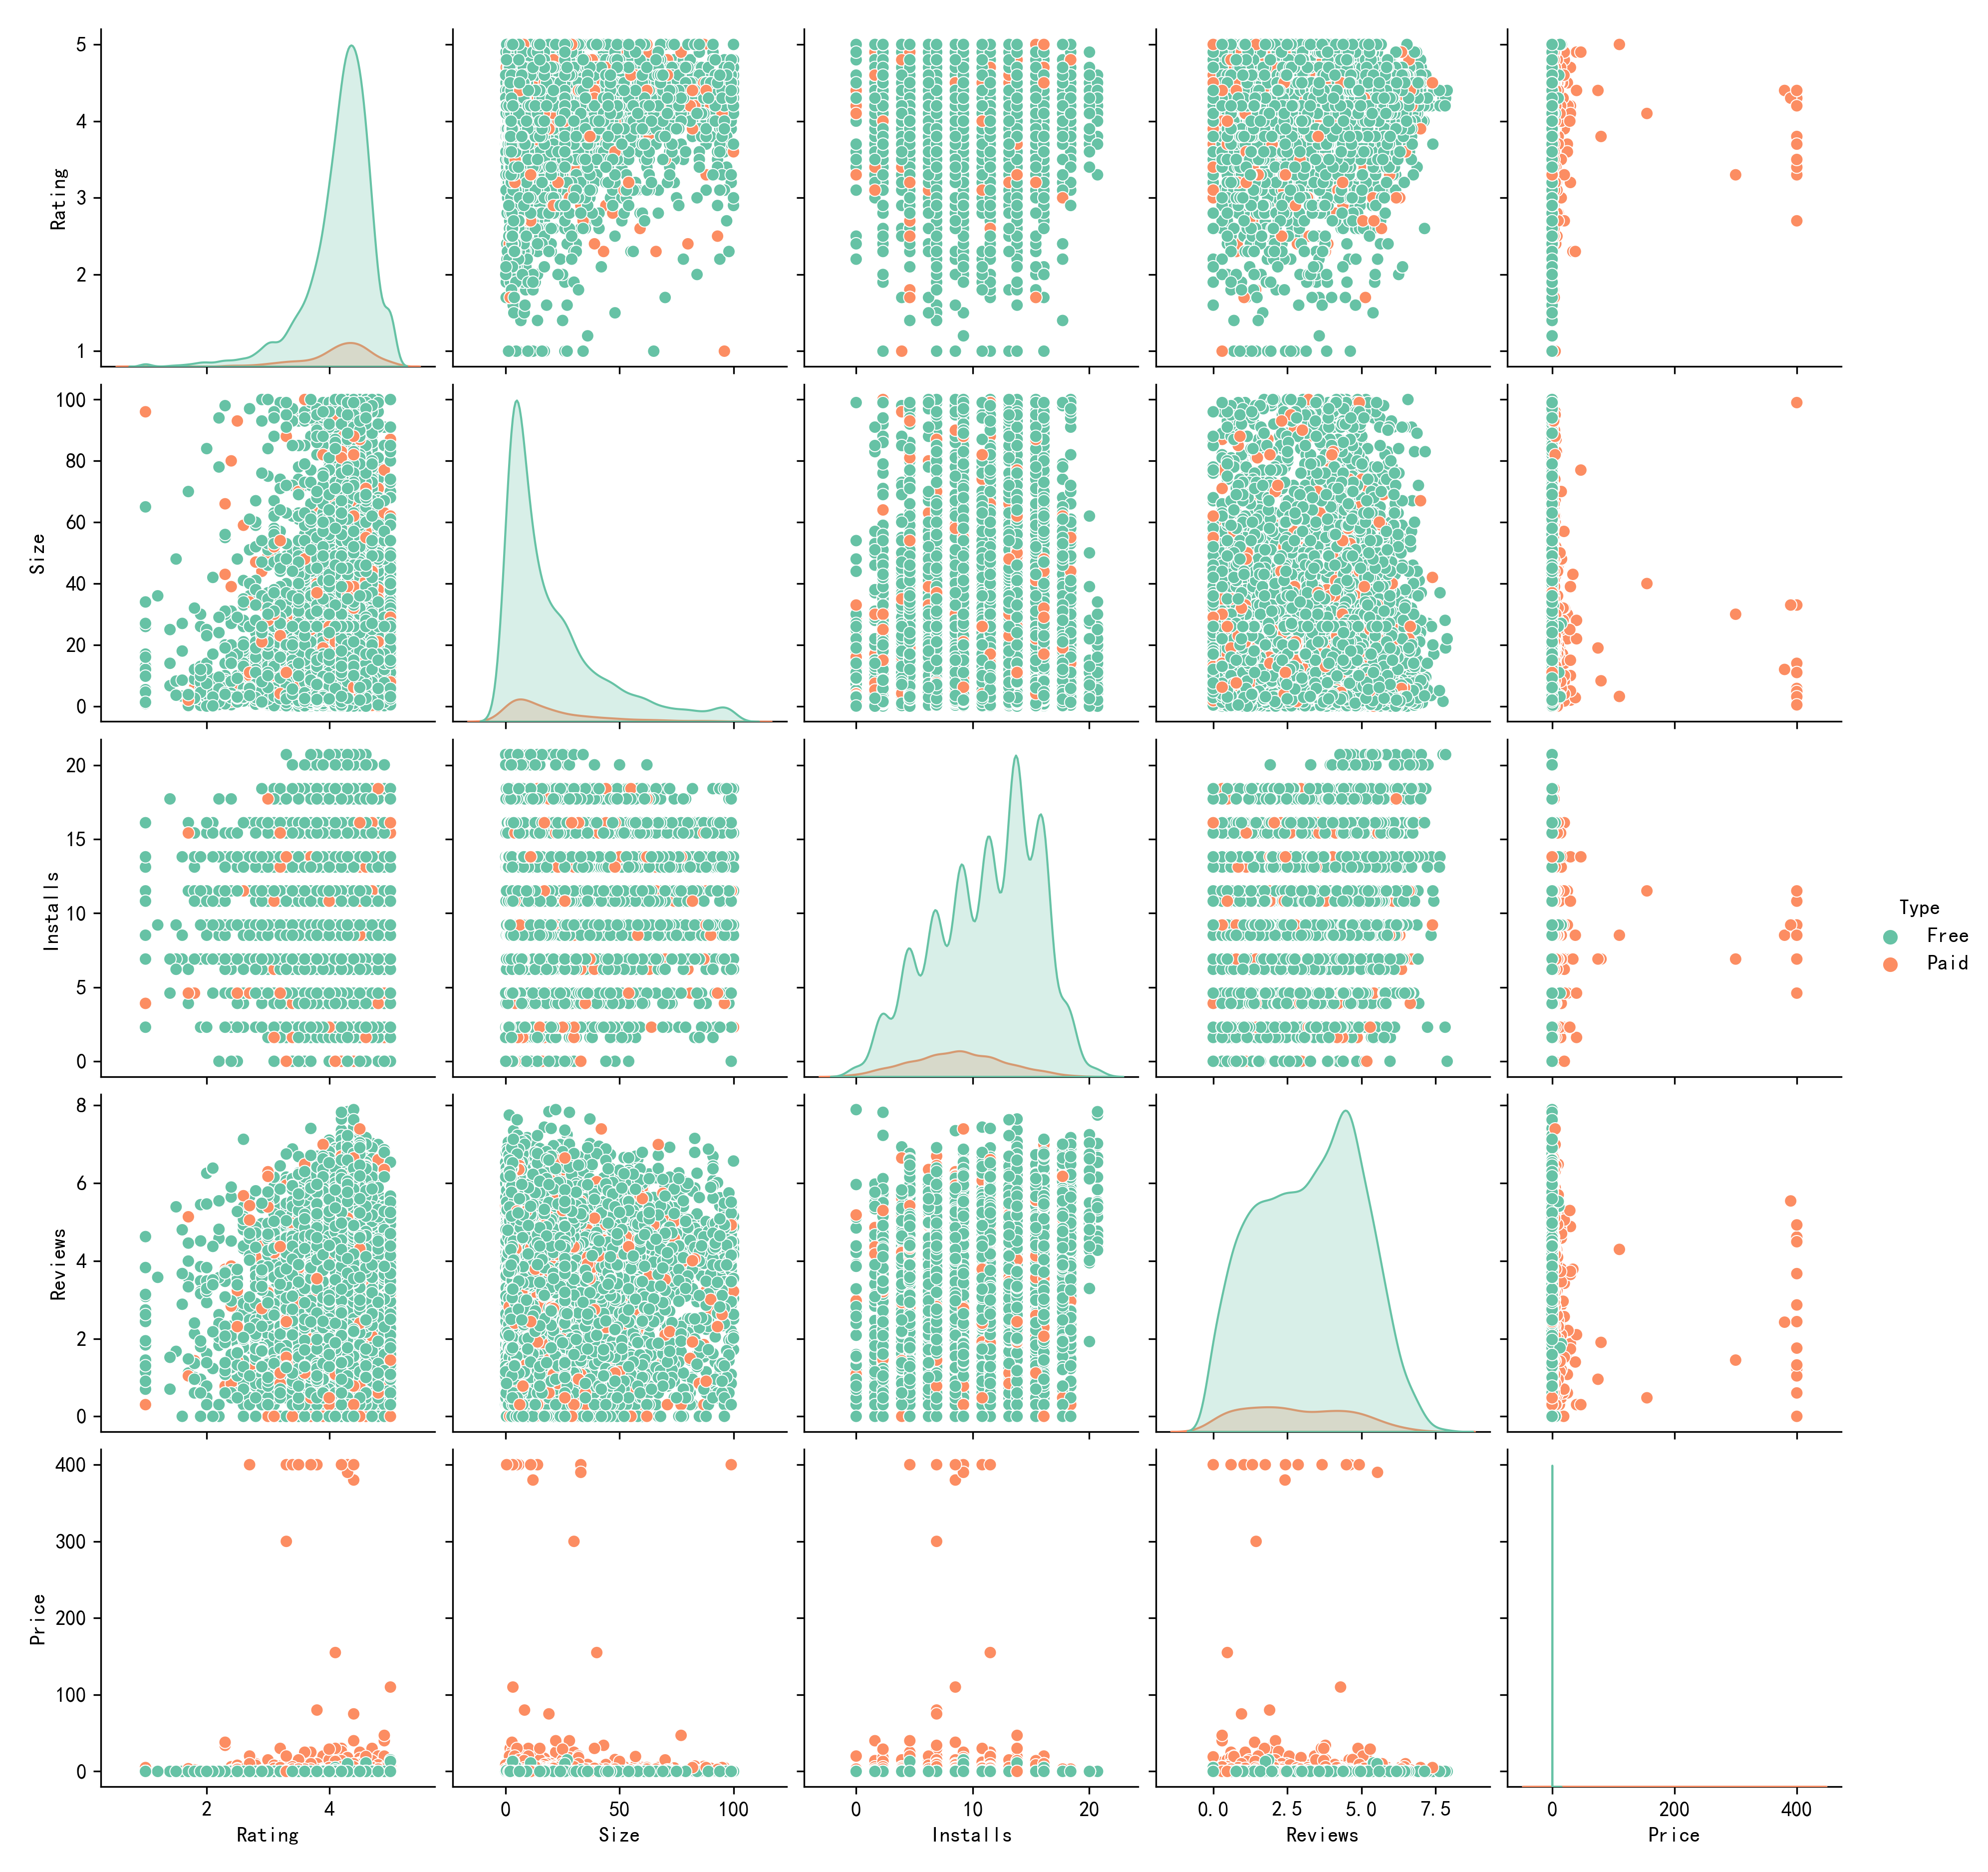
\includegraphics[width=0.8\linewidth]{figures/relation}
	\caption{Relationship}
	\label{fig:Relationship Between}
\end{figure}

\subsubsection{Content Rating}
Box chart, also known as box whisker chart, box chart or box line chart, is a statistical chart used to display a group of data dispersion. It is named for its shape like a box. It is also often used in various fields, common in quality management. It is mainly used to reflect the distribution characteristics of the original data, and can also compare the distribution characteristics of multiple groups of data. The drawing method of boxplot is: first, find out the maximum, minimum, median and two quartiles of a group of data; Then, connect the two quartiles and draw the box; Then connect the maximum and minimum with the box, and the median is in the middle of the box.

I can see a lot of information from the box diagram. Taking content rating as the classification standard and the rating as the ordinate, the free and paid box charts are drawn respectively,and the rating chart is as follows:
\begin{figure}[htbp]
	\centering
	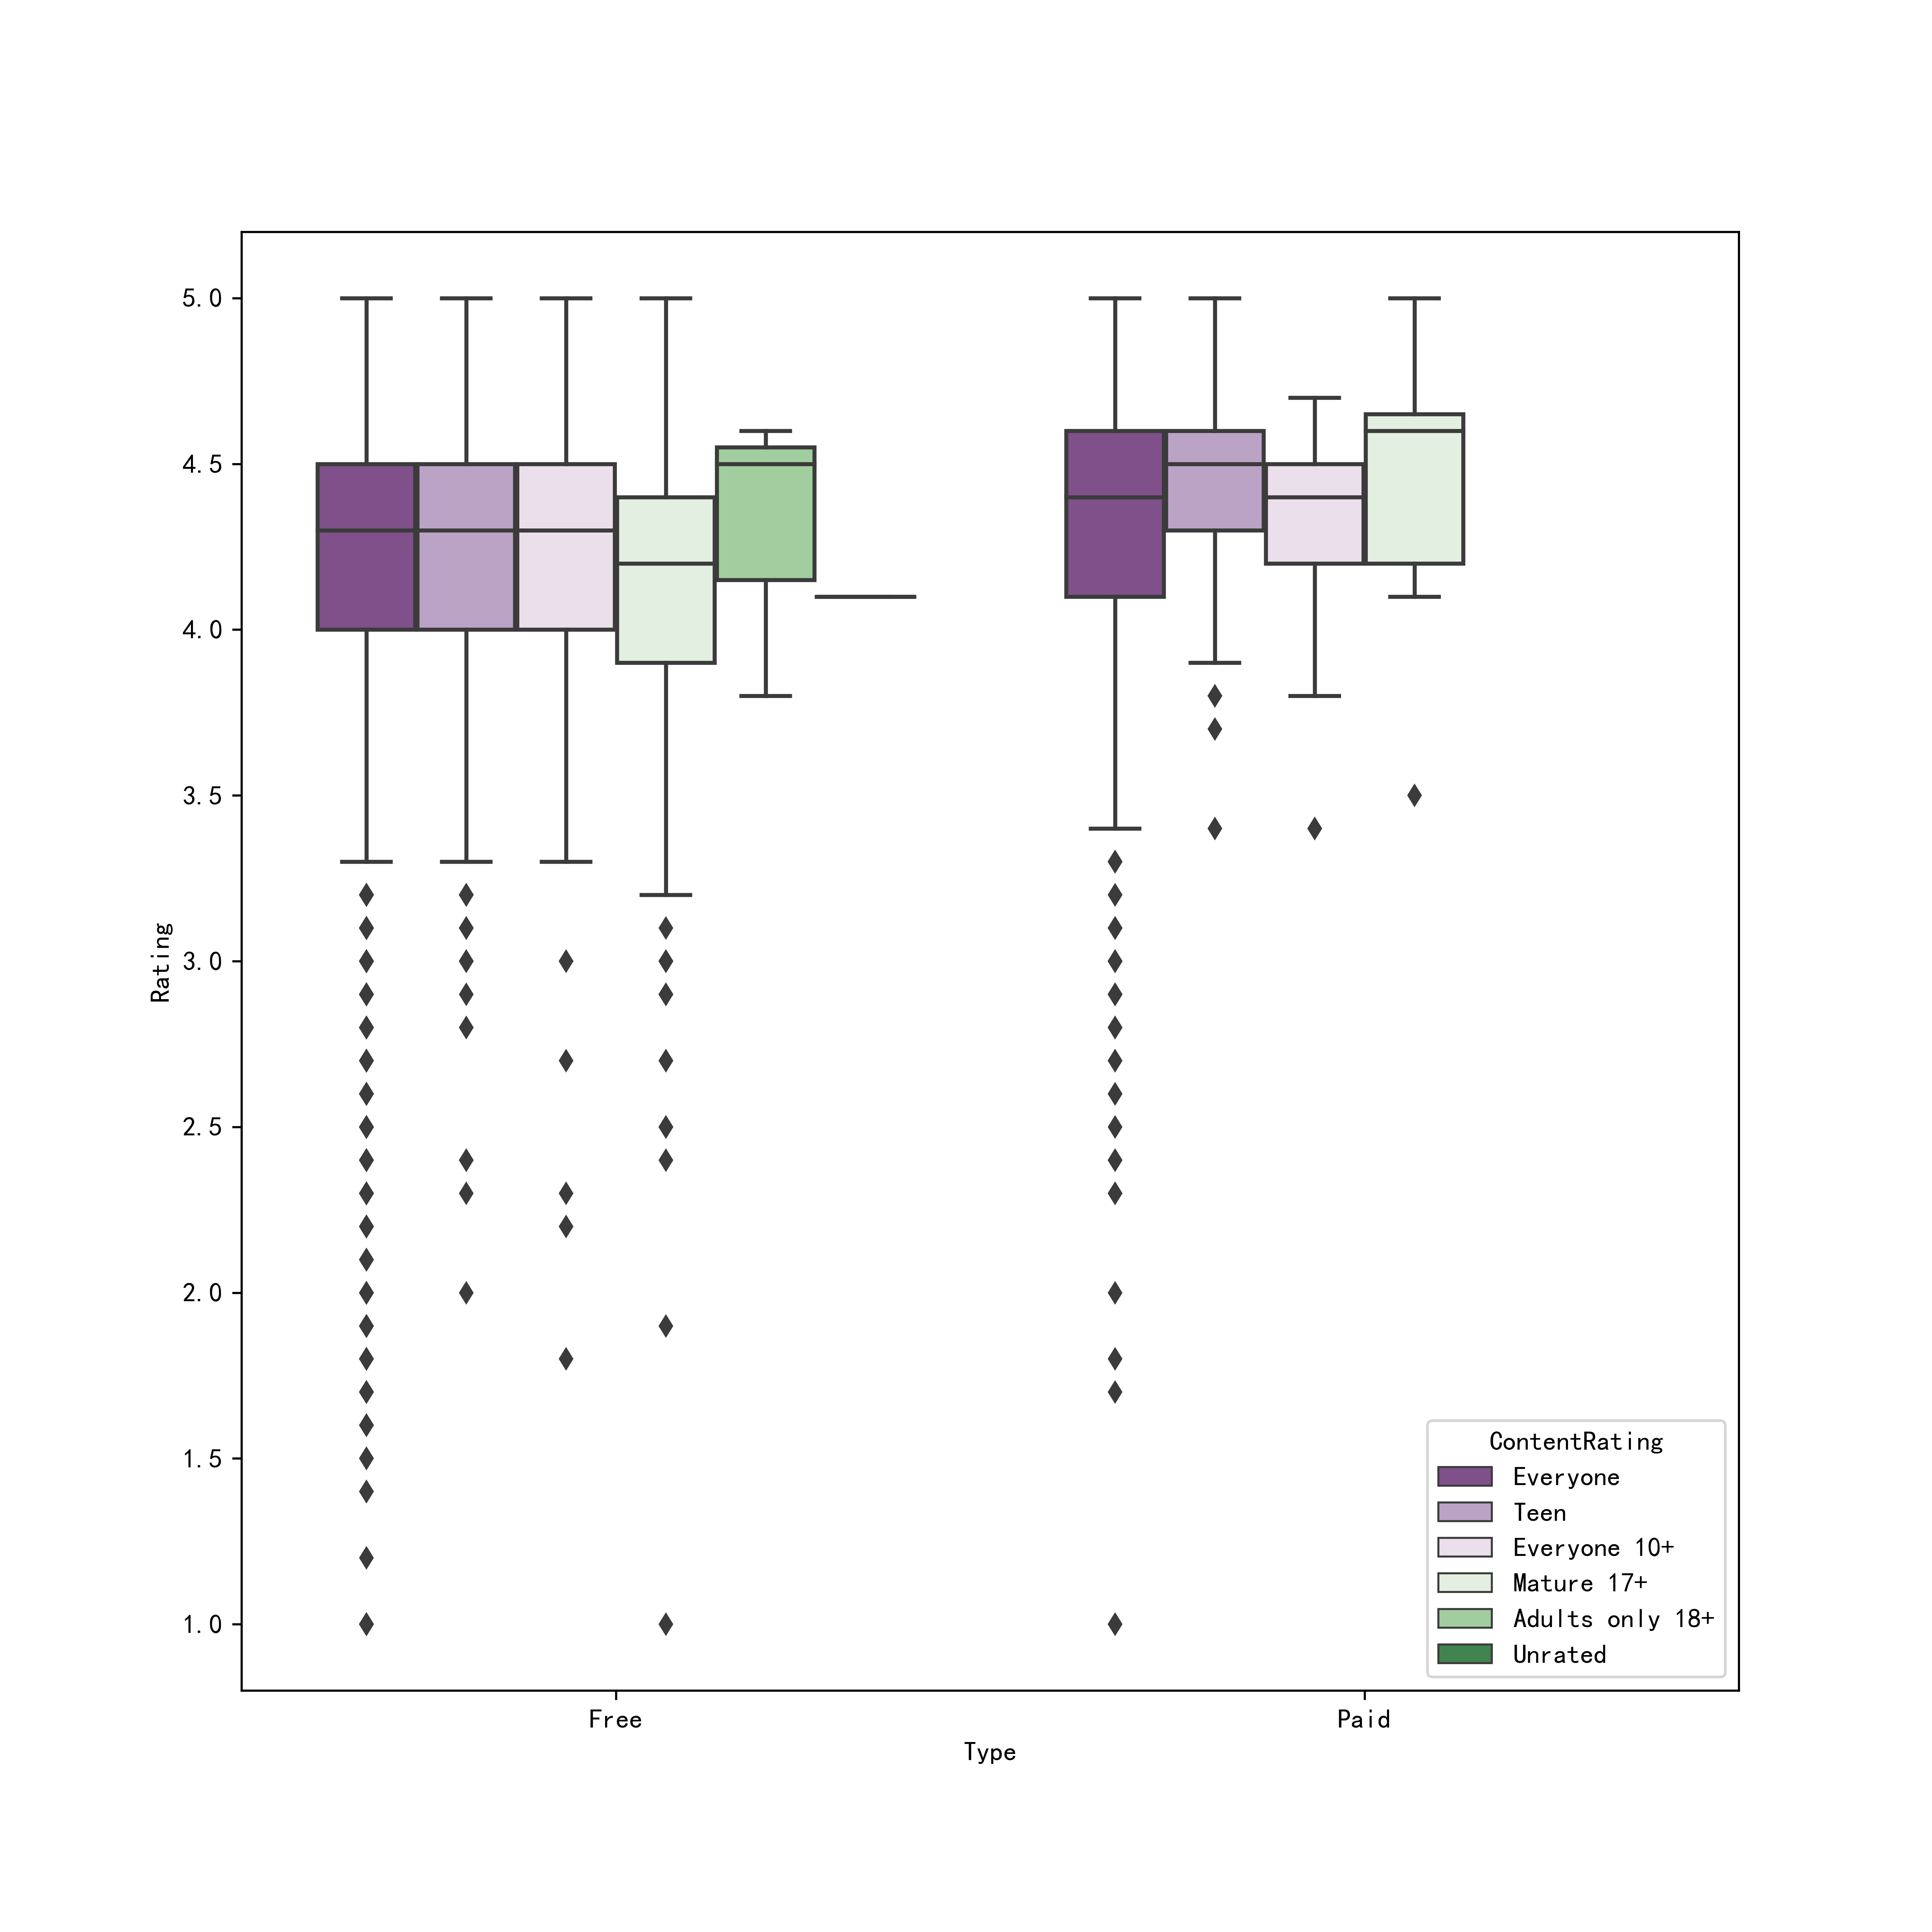
\includegraphics[width=0.7\linewidth]{figures/box}
	\caption{Content Rating with Box Chart}
	\label{fig:contentrating}
\end{figure}
\begin{itemize}
	\item It have six different values in attribute.
	\item I use pie graph to present the relation of content rating and other attributes and information in
	this section.
\end{itemize}
\subsubsection{Price}
\begin{figure}[htbp]
	\centering
	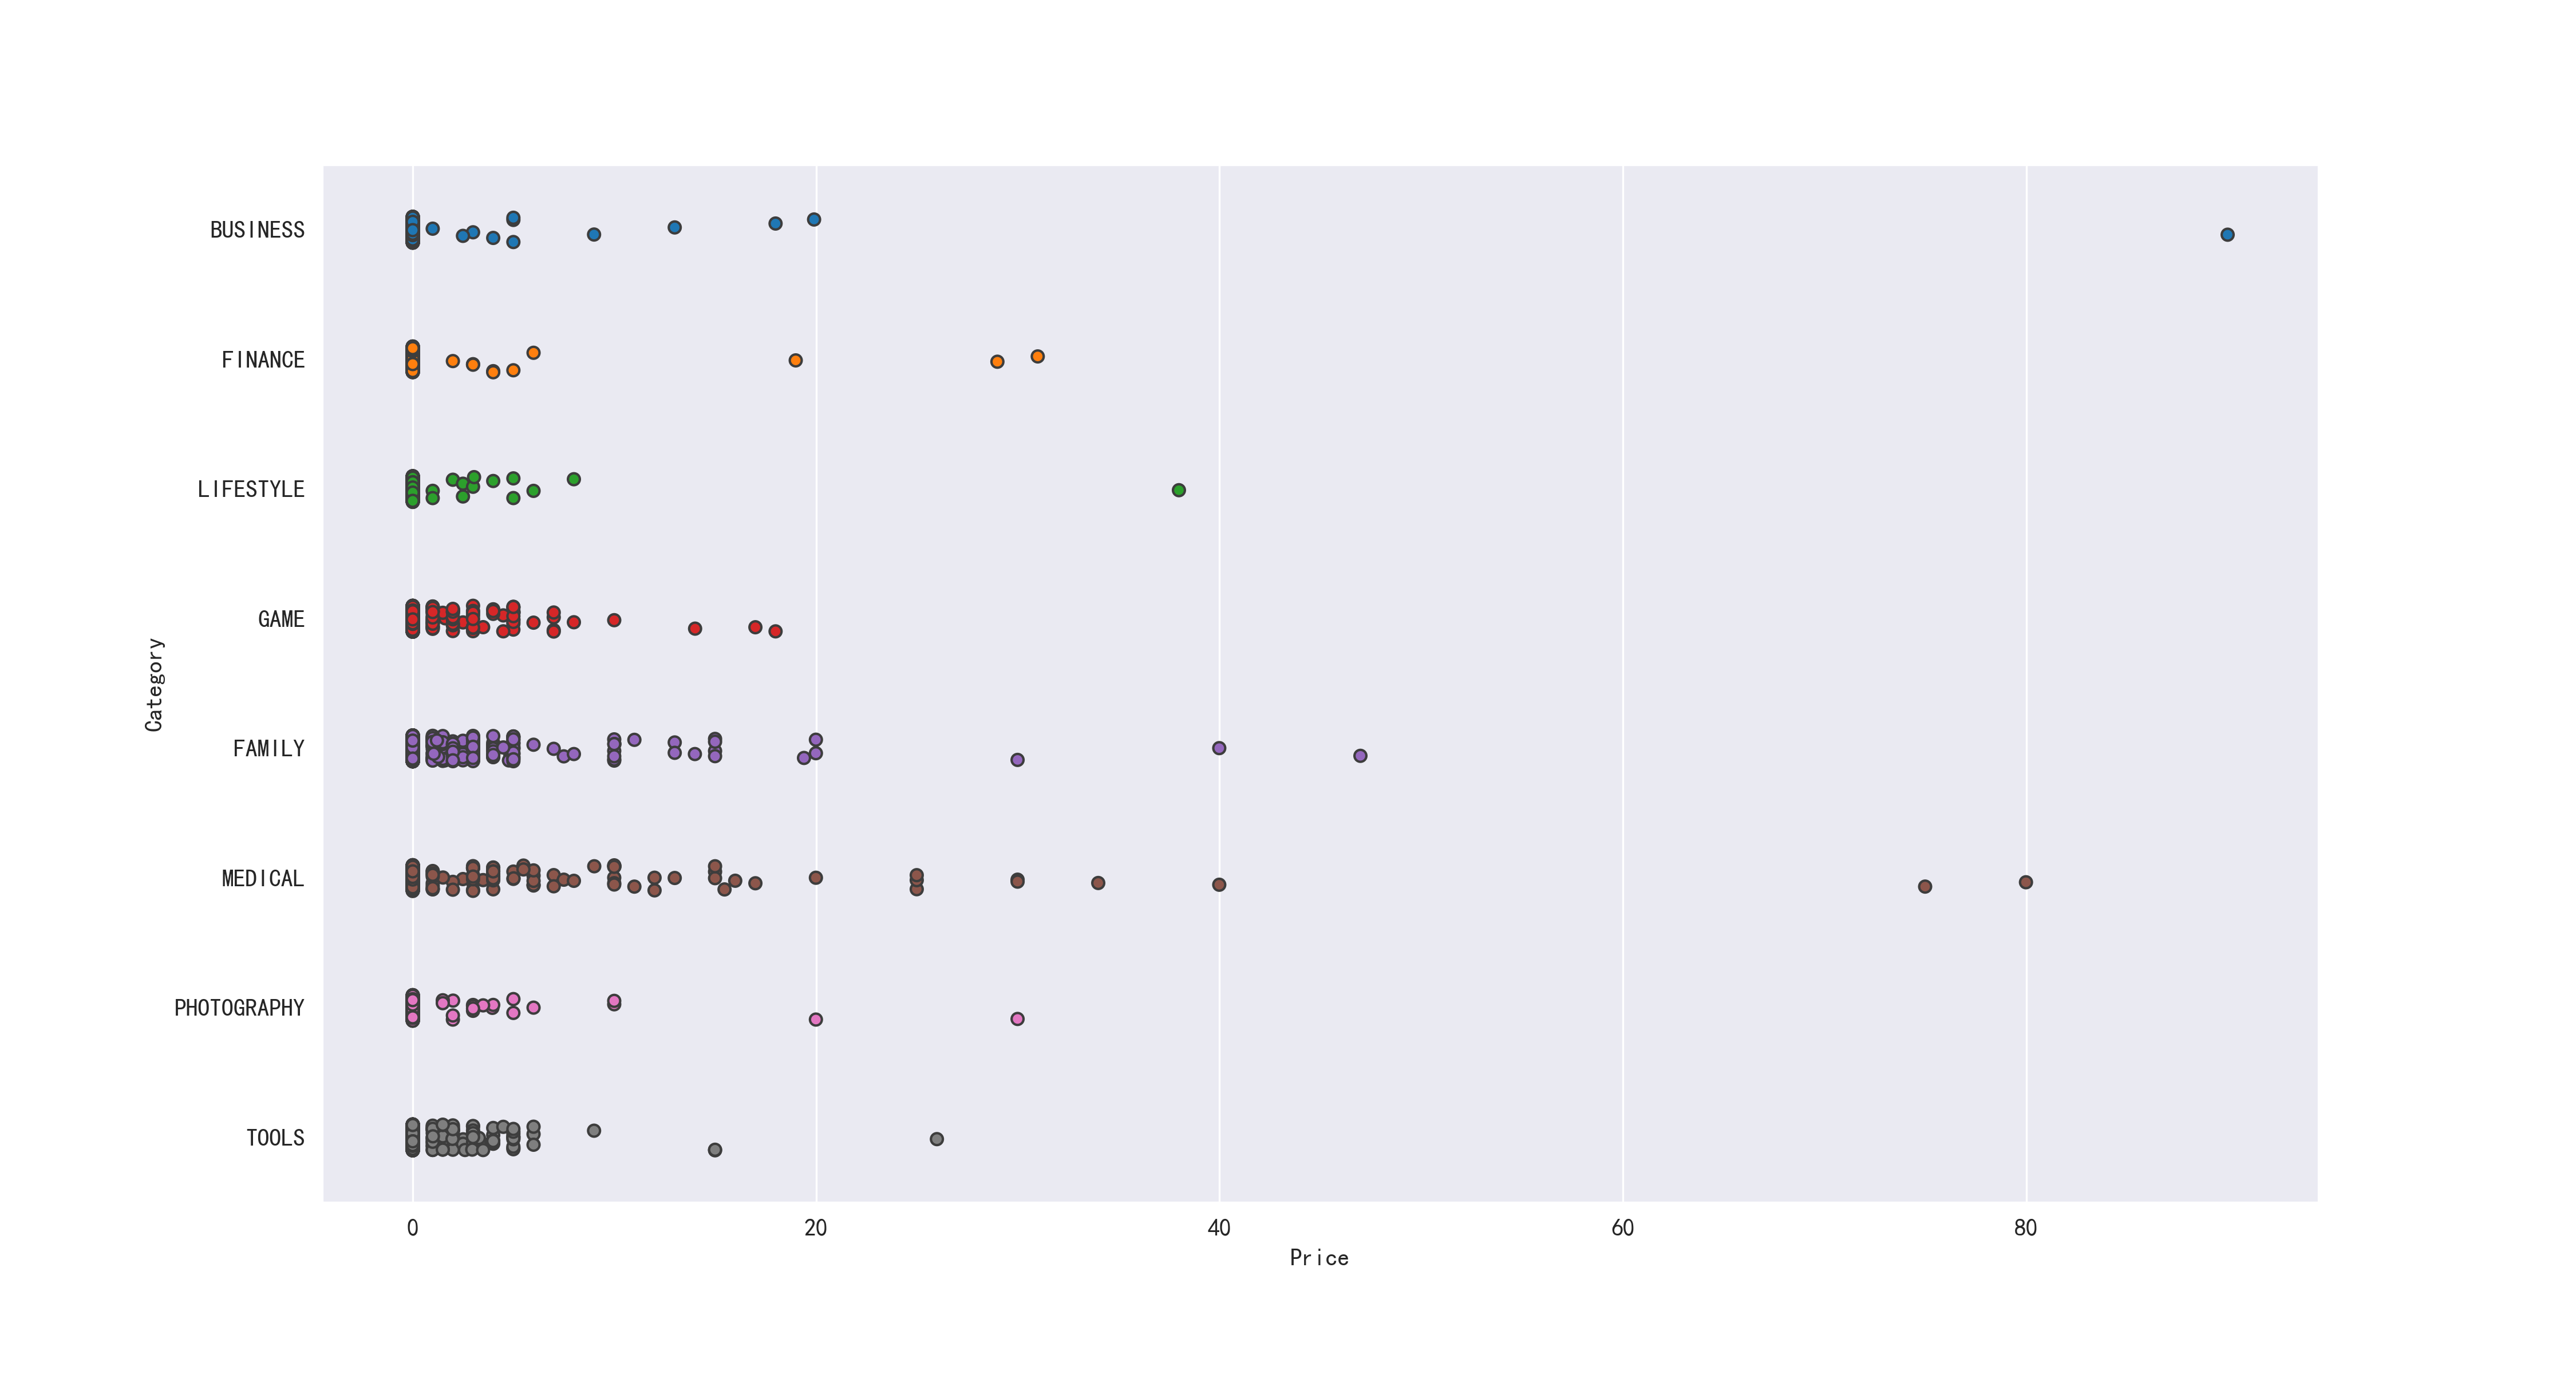
\includegraphics[width=0.7\linewidth]{figures/Price}
	\caption{App Price Distribution}
	\label{fig:Apppricedistribution}
\end{figure}


\begin{itemize}
	\item 0, which means that the App is free for download. And this kind of value is specially.
	\item The price of pharmaceutical apps is very high, and some even reach \$80. What is novel is that the price of game apps is not high, almost no more than \$20.
	
\end{itemize}

\section{Layout of Designed Dashboard}
After I had a general understanding of the data, I started to design my dashboard.I use the suger data visualization framework provided by Baidu to build my big data screen. I've just used three interactive charts to show my data:
scatter, radiation and line column mix-up charts.

\subsection{Interface Design}
The interface overview of my data visualization platform is as show follows:
\begin{figure}[htbp]
	\centering
	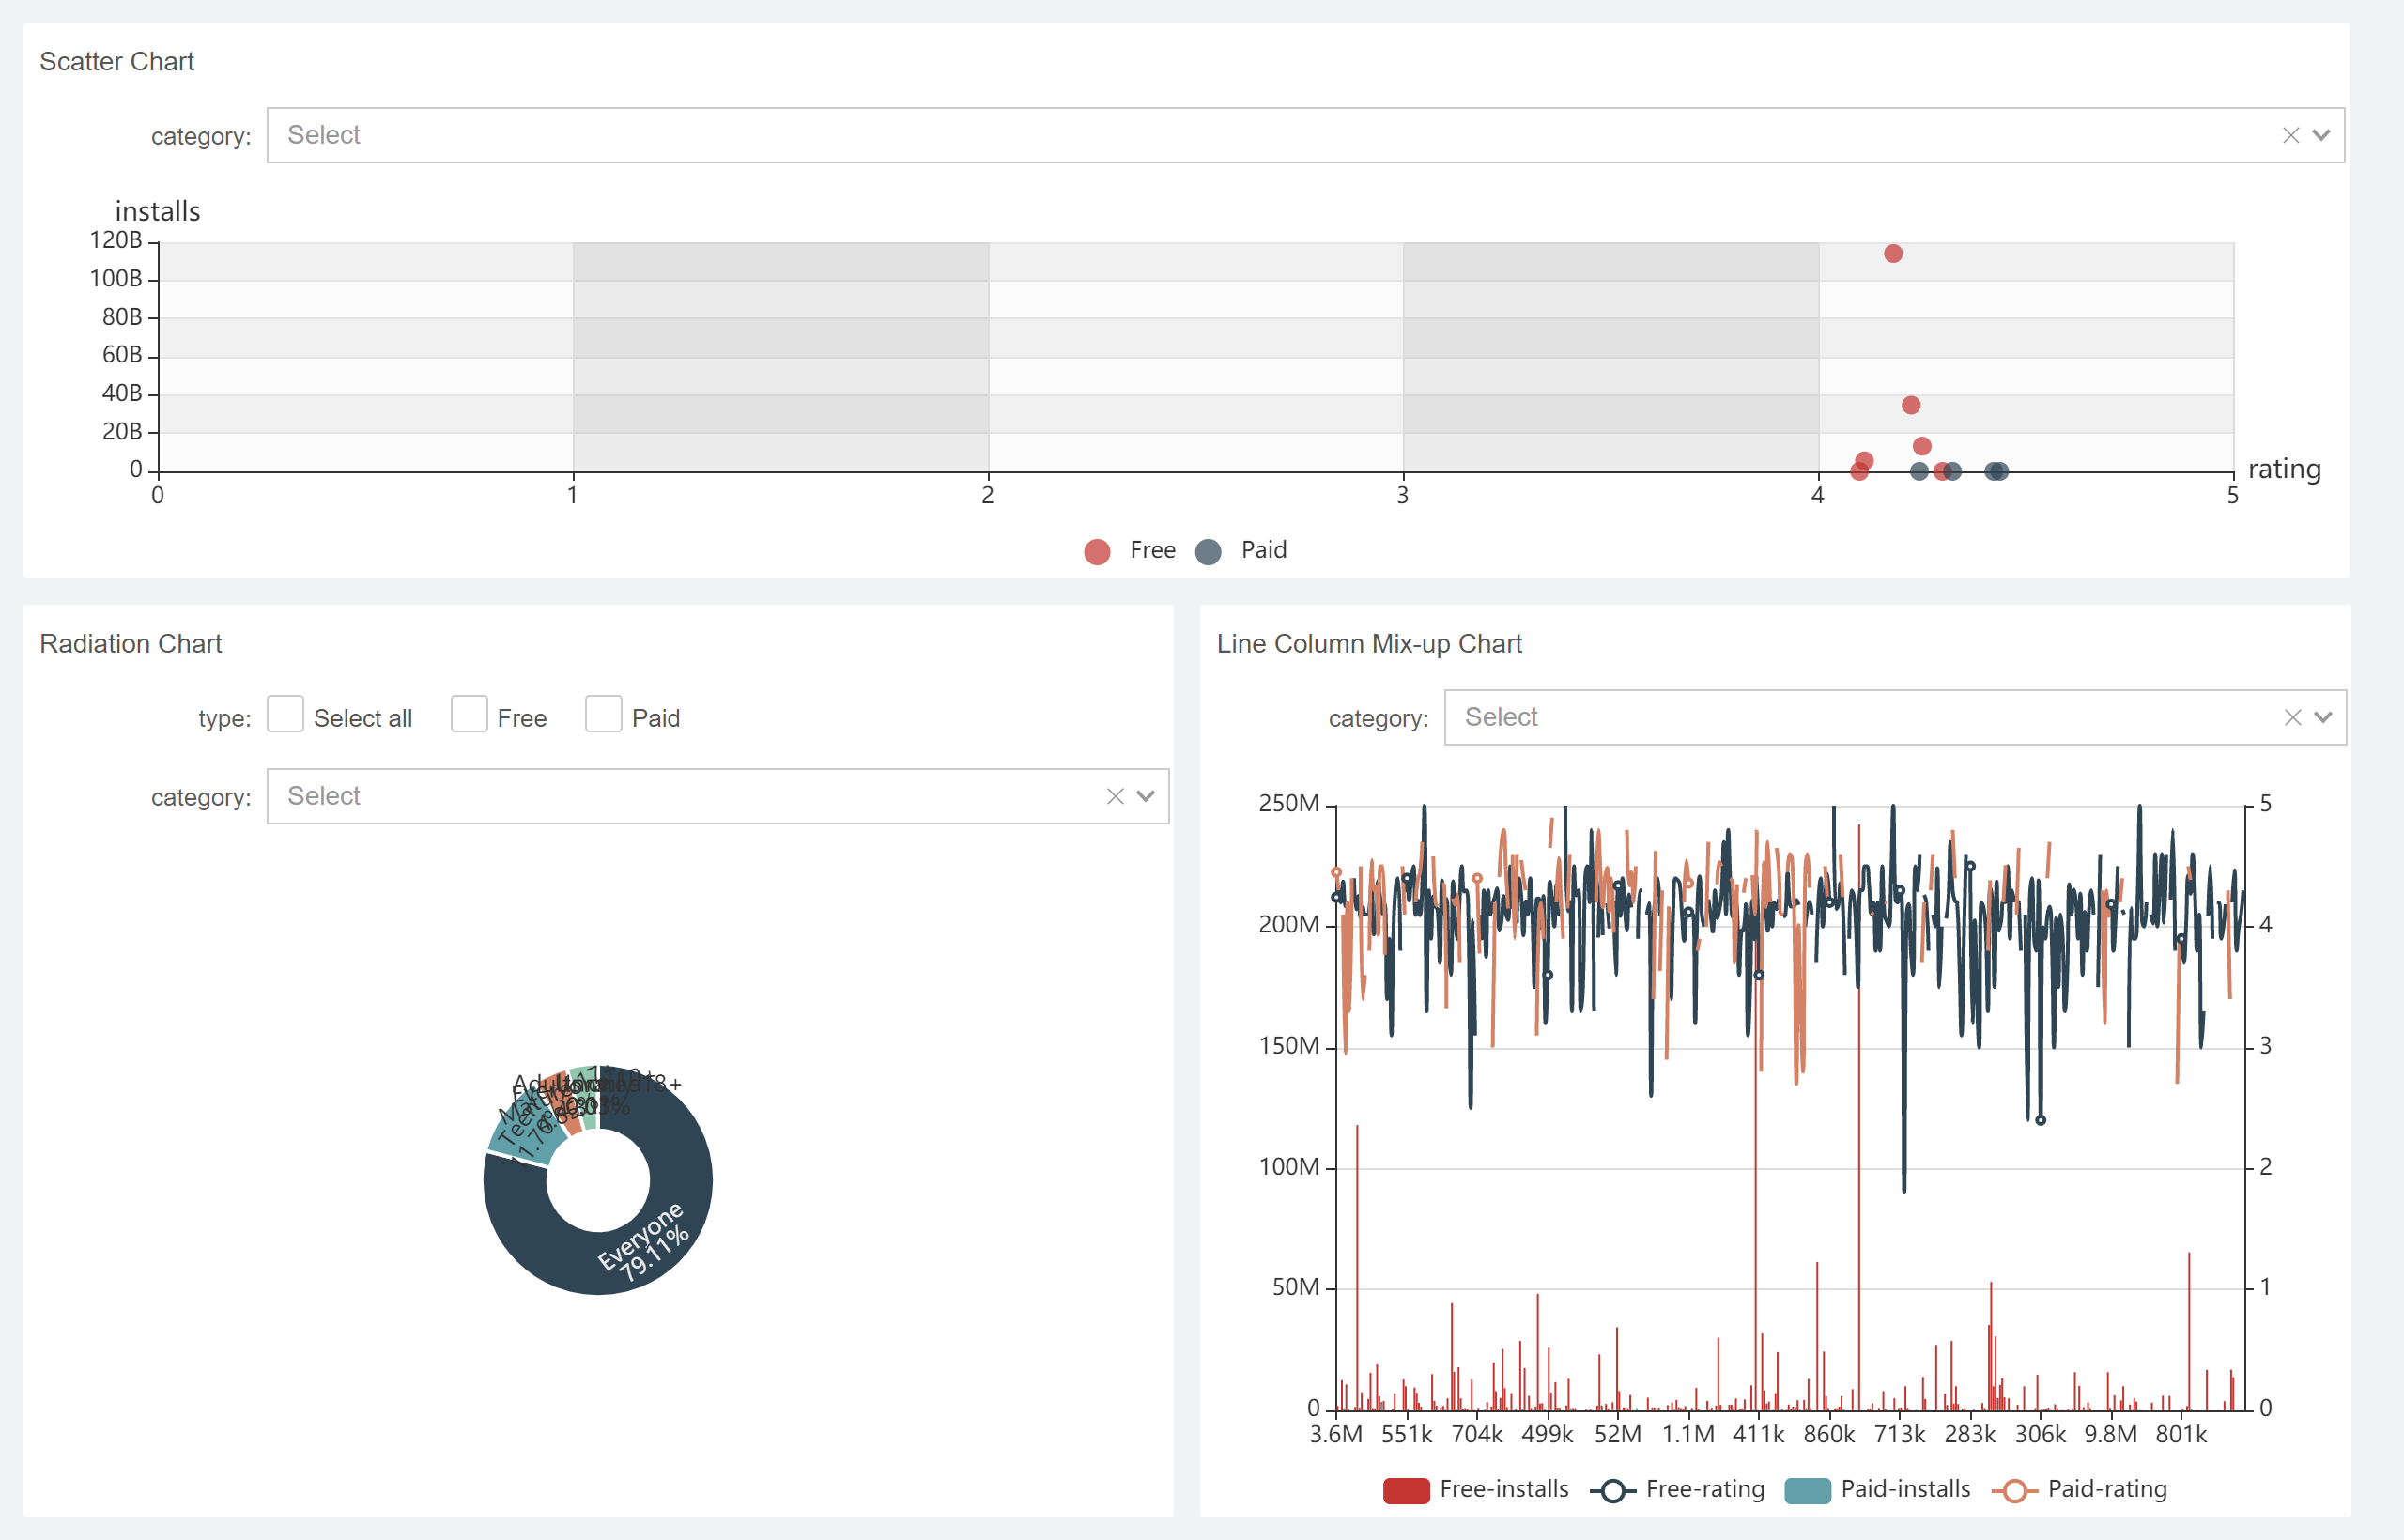
\includegraphics[width=0.8\linewidth]{figures/interface}
	\caption{Data Dashboard Interface}
	\label{fig:interface}
\end{figure}

The three charts are arranged as a triangle.
\subsection{Scatter Chart}
The abscissa of the scatter plot is the average of user ratings, the ordinate is the cumulative sum of user downloads, and the filter is the category of app.The two color tags represent paid apps and free apps.
\begin{figure}[htbp]
	\centering
	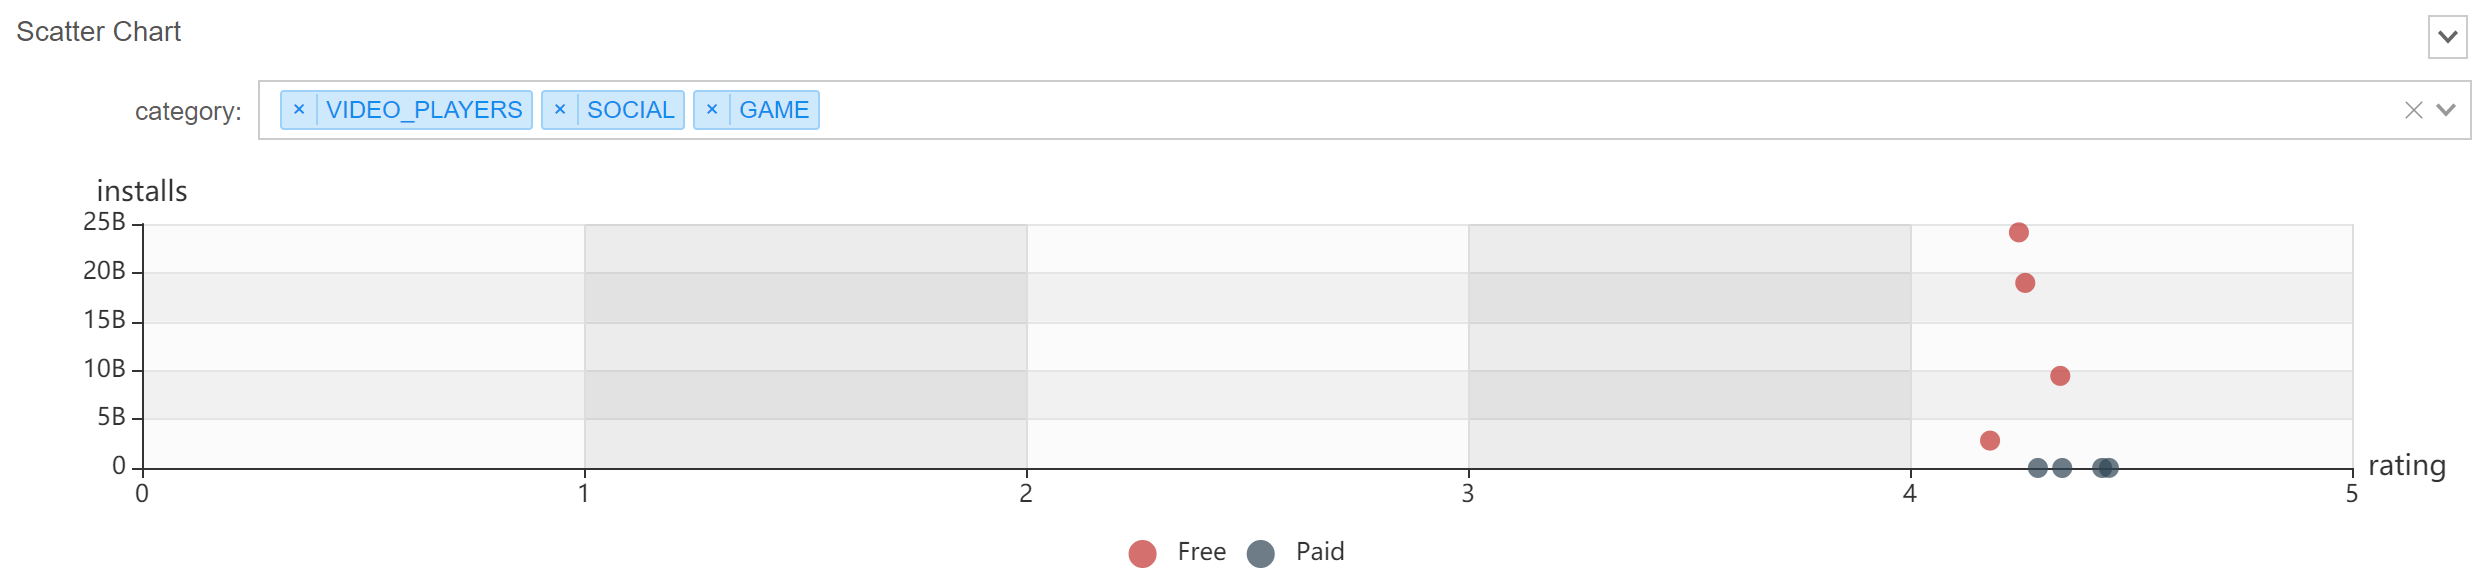
\includegraphics[width=0.8\linewidth]{figures/scatter}
	\caption{Scatter Chart}
	\label{fig:Scatter Chart}
\end{figure}

You can click the down button to start the drawer to select category of app you want.
\begin{figure}[htbp]
	\centering
	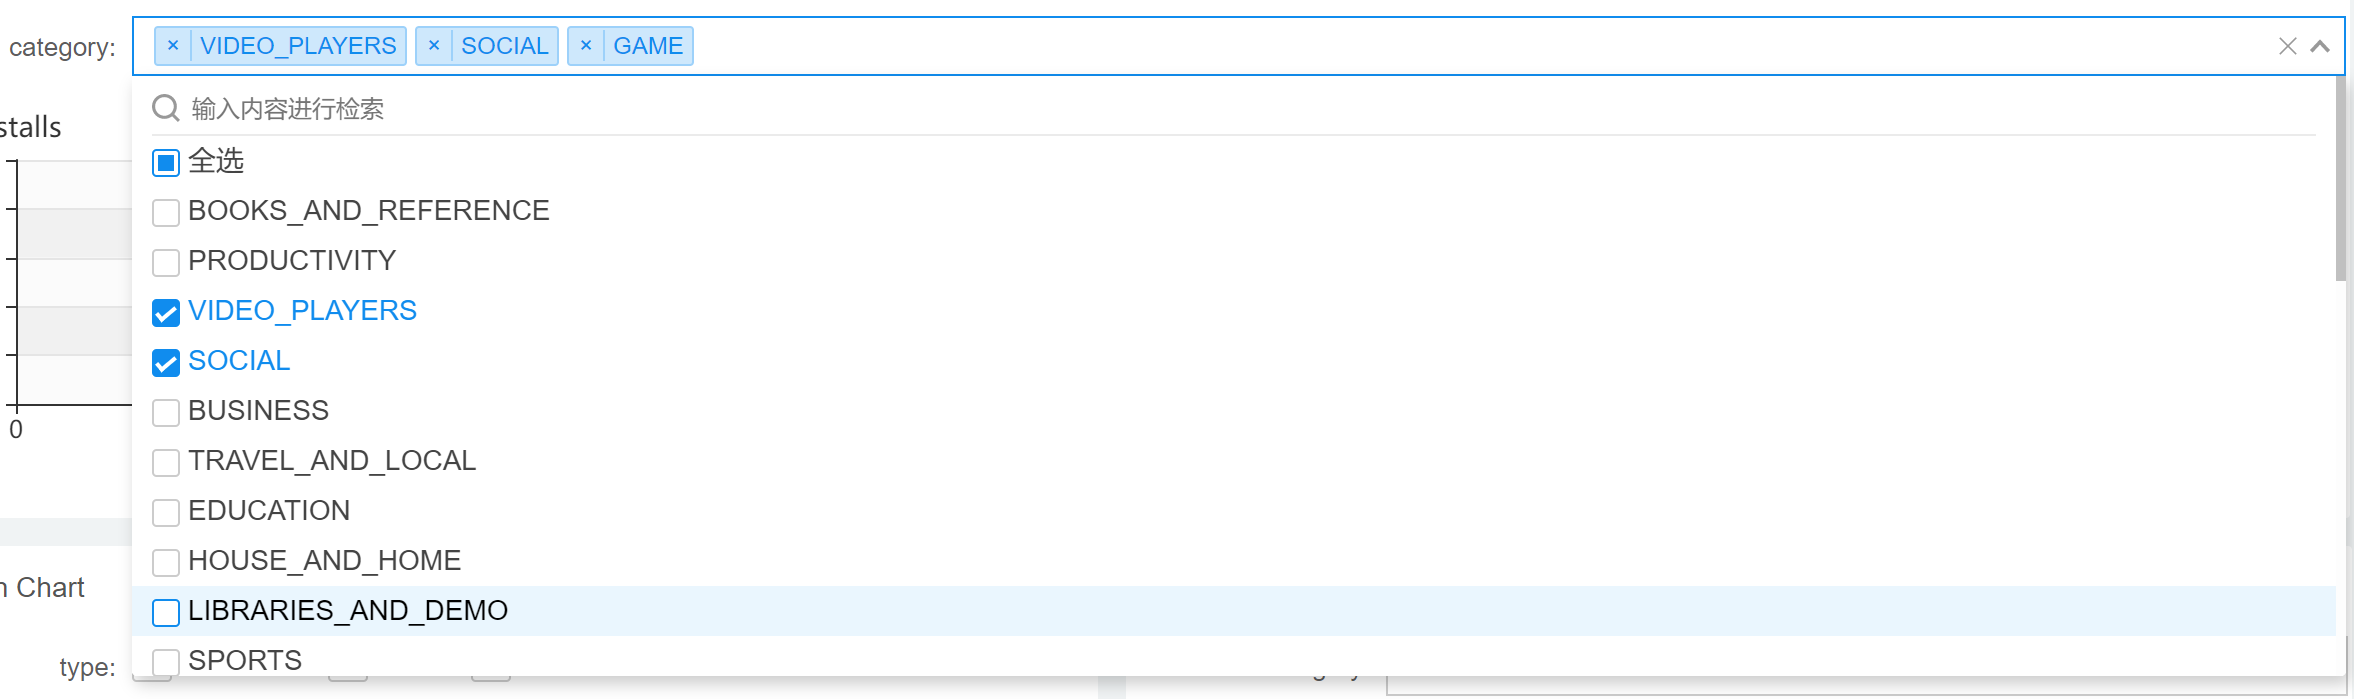
\includegraphics[width=0.8\linewidth]{figures/filter}
	\caption{Use Filter}
	\label{fig:filter}
\end{figure}

\subsection{Radiation Chart}
Radiation chart reflects the distribution of various content rating apps in different app category.
\begin{figure}[htbp]
	\centering
	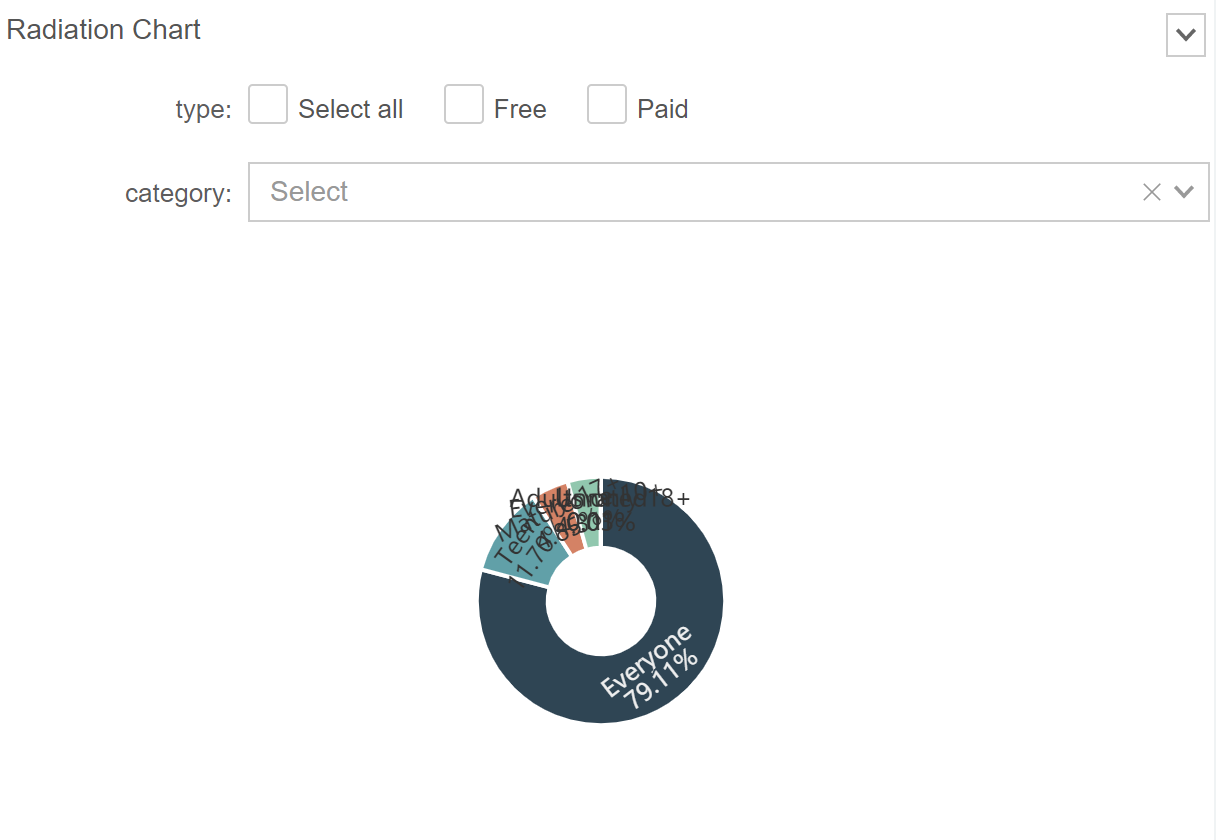
\includegraphics[width=0.7\linewidth]{figures/RadiationChart}
	\caption{Radiation Chart}
	\label{fig:RadiationChart}
\end{figure}

Similar to the scatter plot, you can use the drop-down drawer component to select filters and can use the check box to select app type.

The chart is interactive. You can move the mouse over a color block in the chart, and then the chart will display the details of the color block.
\begin{figure}[htbp]
	\centering
	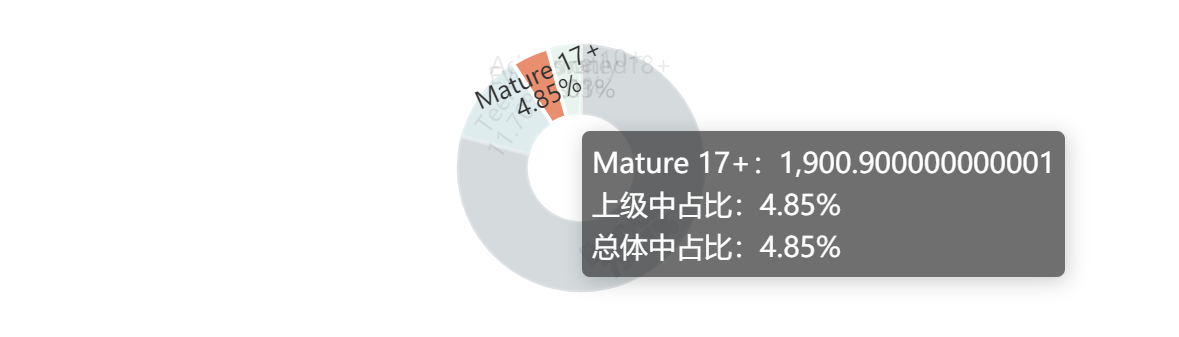
\includegraphics[width=0.7\linewidth]{figures/inter}
	\caption{Interactive Function}
	\label{fig:InterChart}
\end{figure}

\subsection{Line Column Mix-up Chart}
The x-axis of this mixed chart is the size of the app, and the vertical axis is the download amount and rating of the app.Similar to the scatter plot, you can use the drop-down drawer component to select filters.
\begin{figure}[htbp]
	\centering
	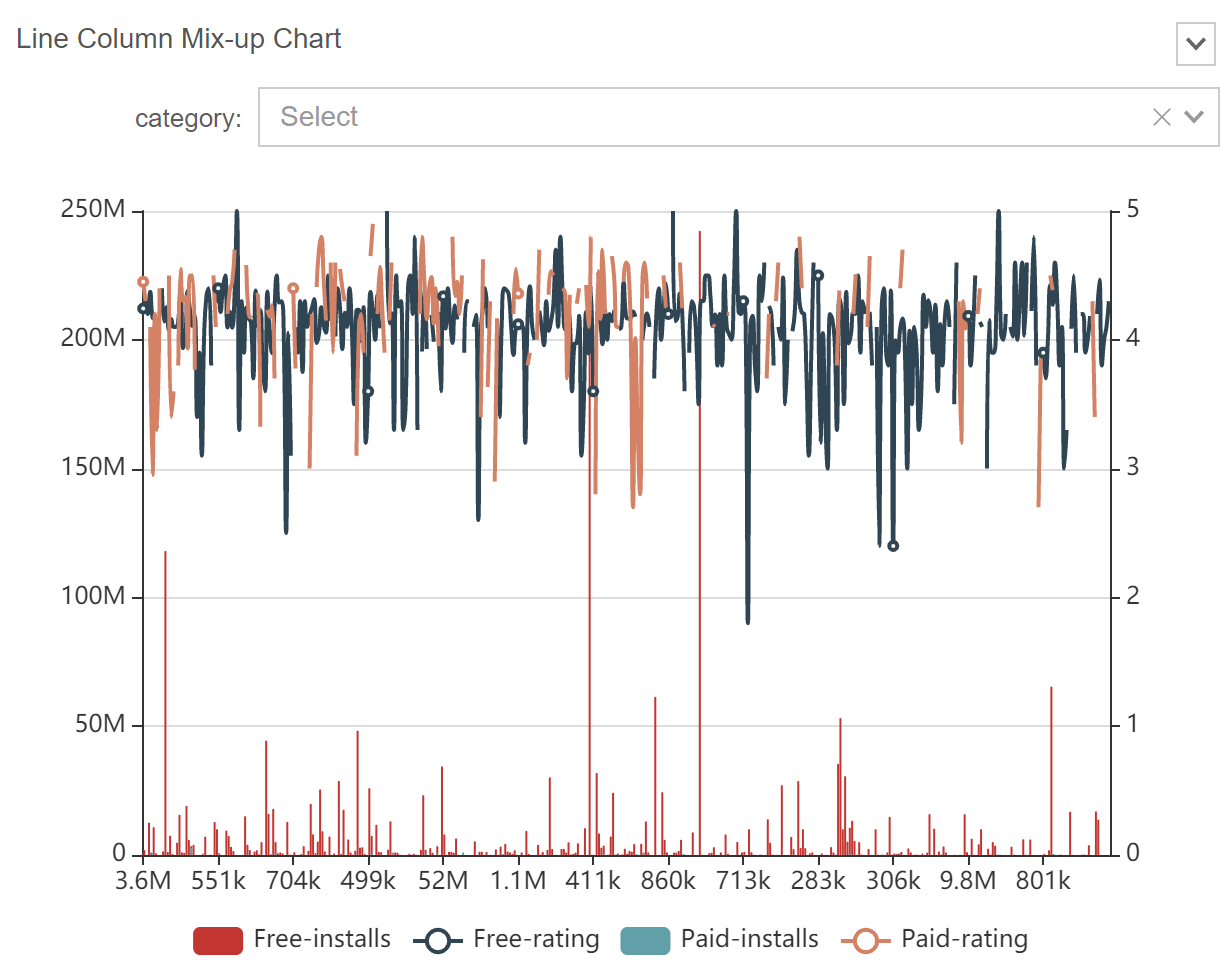
\includegraphics[width=0.7\linewidth]{figures/LineColumnMix-upChart}
	\caption{Line Column Mix-up Chart}
	\label{fig:Line Column Mix-up Chart}
\end{figure}

Move the mouse over the chart to display the selected data.
\begin{figure}[htbp]
	\centering
	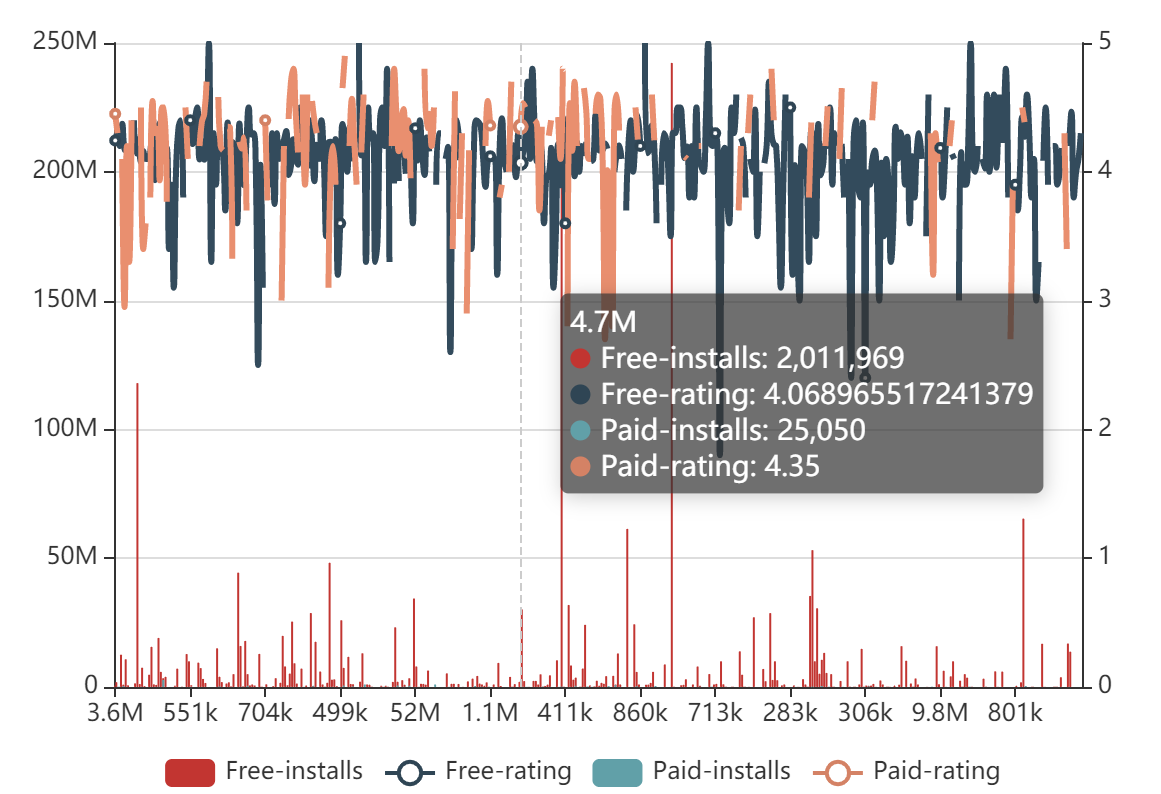
\includegraphics[width=0.7\linewidth]{figures/inter1}
	\caption{Interactive Function}
	\label{fig:inter}
\end{figure}
\subsection{Deployment}
The data dashboard is deployed on a cloud server, and you can access it by scanning the QR code below.
\begin{figure}[htbp]
	\centering
	
\includegraphics[width=0.3\linewidth]{figures/QR}
	\caption{QR Code}
	\label{fig:QR}
\end{figure}





\begin{thebibliography}{99}
\bibitem{1} Designing the User Interface: Strategies for Effective Human-Computer Interaction, 6th edition,Ben Shneiderman,Catherine Plaisant,Maxine Cohen
\bibitem{2} Baidu Data Visualization Sugar,  \url{https://cloud.baidu.com/doc/SUGAR/index.html}
\end{thebibliography}

\end{document}
%%
%% This work consists of these files mcmthesis.dtx,
%%                                   figures/ and
%%                                   code/,
%% and the derived files             mcmthesis.cls,
%%                  command execution                 mcmthesis-demo.tex,
%%                                   README,
%%                                   LICENSE,
%%                                   mcmthesis.pdf and
%%                                   mcmthesis-demo.pdf.
%%
%% End of file `mcmthesis-demo.tex'.
